\documentclass[11pt, a4paper]{article}

% Mandatory Packages
\usepackage{amsmath}
\usepackage{amssymb}
\usepackage{amsthm}
\usepackage{geometry}
\usepackage{tikz}
\usepackage{mathrsfs}
\usepackage{mathtools}
\usepackage{hyperref}
\usepackage{enumitem}

% TikZ Libraries
\usetikzlibrary{arrows.meta, positioning, shapes, backgrounds}

% Page Geometry
\geometry{top=1in, bottom=1in, left=1in, right=1in}

% Theorem Environments
\newtheorem{theorem}{Theorem}[section]
\newtheorem{lemma}[theorem]{Lemma}
\newtheorem{proposition}[theorem]{Proposition}
\newtheorem{corollary}[theorem]{Corollary}
\theoremstyle{definition}
\newtheorem{definition}{Definition}[section]
\newtheorem{example}{Example}[section]
\theoremstyle{remark}
\newtheorem{remark}{Remark}[section]

% Custom Commands
\newcommand{\R}{\mathbb{R}}
\newcommand{\N}{\mathbb{N}}
\newcommand{\Z}{\mathbb{Z}}
\newcommand{\Q}{\mathbb{Q}}
\newcommand{\E}{\mathbb{E}}
\newcommand{\Prob}{\mathbb{P}}
\newcommand{\F}{\mathcal{F}}

% Title Information
\title{\textbf{Homework 5: Existence Proofs and Disproving Existence Statements}}
\author{Tashfeen Omran}
\date{September 2026}

\begin{document}

\maketitle
\tableofcontents
\newpage

% ==========================================
% PART 1: INTRODUCTION
% ==========================================
\section{Part 1: Comprehensive Introduction, Context, and Prerequisites}

\subsection{Core Concepts \& Axioms}
In advanced abstract mathematics, establishing the truth of a proposition often boils down to verifying the existence (or non-existence) of a mathematical object satisfying a specific property. This chapter focuses on two logically inverse operations:
\begin{enumerate}
    \item \textbf{Existence Proofs ($\exists x \in S, P(x)$):} Demonstrating that within a given domain $S$, there is at least one element $x$ for which the open sentence $P(x)$ is true.
    \item \textbf{Disproving Existence Statements ($\sim[\exists x \in S, P(x)]$):} Demonstrating that no such element exists. By De Morgan's Laws for Quantifiers, this is logically equivalent to proving the universal statement $\forall x \in S, \sim P(x)$.
\end{enumerate}

Existence proofs generally fall into two categories:
\begin{itemize}
    \item \textbf{Constructive Proofs:} We explicitly produce an example $x = c$ and verify that $P(c)$ holds.
    \item \textbf{Non-Constructive Proofs:} We prove that such an $x$ \textit{must} exist due to overarching axioms or theorems (like the Intermediate Value Theorem or the Pigeonhole Principle), without ever identifying the specific value of $x$.
\end{itemize}

\subsection{Intuition and Set-Theoretic Foundations}
Imagine a sample space $\Omega$ and a subset $A \subset \Omega$ defined by $A = \{x \in \Omega : P(x) \text{ is true}\}$. 
An existence proof is equivalent to showing that the measure of $A$ is non-zero, or simply that $A \neq \emptyset$. Disproving existence is equivalent to showing $A = \emptyset$, which requires proving that its complement $A^c = \Omega$. Constructive existence is akin to pulling a specific element out of $A$ and showing it to the reader. Non-constructive existence is akin to weighing the set $A$ and showing its mass is strictly positive, guaranteeing it cannot be empty.

\subsection{Historical Context and Motivation}
The debate between constructive and non-constructive existence proofs triggered the foundational crisis of mathematics in the early 20th century. L.E.J. Brouwer championed \textit{Intuitionism}, arguing that mathematical objects only exist if they can be explicitly constructed. David Hilbert, defending classical logic, argued that denying non-constructive proofs (like those relying on the Law of Excluded Middle) would "deny the astronomer the telescope." Today, classical mathematics accepts non-constructive proofs, which are foundational to modern probability theory and measure theory (e.g., the existence of non-measurable sets via the Axiom of Choice).

\subsection{Key Theorems and Logical Equivalences}
\begin{theorem}[De Morgan's Laws for Quantifiers]
    \[ \sim(\exists x \in S, P(x)) \equiv \forall x \in S, \sim P(x) \]
    \[ \sim(\forall x \in S, P(x)) \equiv \exists x \in S, \sim P(x) \]
\end{theorem}

\begin{theorem}[Intermediate Value Theorem (IVT)]
    Let $f: [a, b] \to \R$ be a continuous function. If $k$ is a real number strictly between $f(a)$ and $f(b)$, then $\exists c \in (a, b)$ such that $f(c) = k$.
\end{theorem}

\begin{theorem}[Pigeonhole Principle]
    If $n$ items are put into $m$ containers, with $n > m$, then at least one container must contain more than one item.
\end{theorem}

\subsection{Prerequisites}
To master this section, one must be fluent in:
\begin{itemize}
    \item \textbf{Modular Arithmetic:} Essential for restricting domains in non-existence proofs.
    \item \textbf{Real Analysis:} Basic continuity and the Intermediate Value Theorem.
    \item \textbf{Proof by Contradiction:} The primary engine for disproving existence.
    \item \textbf{Strong Induction:} Required for proving existence over the natural numbers (e.g., the Frobenius coin problem).
\end{itemize}

\newpage

% ==========================================
% PART 2: DETAILED HOMEWORK SOLUTIONS
% ==========================================
\section{Part 2: Detailed Homework Solutions}

\subsection{Section 5.4: Existence Proofs}

\textbf{Problem 5.42:} Show that there exist a rational number $a$ and an irrational number $b$ such that $a^b$ is rational.
\begin{proof}[Proof (Constructive)]
    Let $a = 2$, which is clearly a rational number. Let $b = \log_2(3)$. 
    First, we must prove $b$ is irrational. Assume for contradiction that $\log_2(3) = \frac{p}{q}$ for some $p, q \in \Z^+$ with $q \neq 0$. Then $2^{p/q} = 3$, which implies $2^p = 3^q$. Since $p, q > 0$, the left side is an even integer and the right side is an odd integer. This is a contradiction. Thus, $b = \log_2(3)$ is irrational.
    Now, evaluate $a^b$:
    \[ a^b = 2^{\log_2(3)} = 3 \]
    Since $3$ is a rational number, we have found a rational $a$ and irrational $b$ such that $a^b$ is rational.
\end{proof}

\textbf{Problem 5.43:} Show that there exist a rational number $a$ and an irrational number $b$ such that $a^b$ is irrational.
\begin{proof}[Proof (Constructive)]
    Let $a = 2$, which is rational. Let $b = \log_2(\sqrt{3})$. 
    First, we prove $b$ is irrational. Assume $\log_2(\sqrt{3}) = \frac{p}{q}$ for $p, q \in \Z^+$. Then $2^{p/q} = \sqrt{3} \implies 2^{2p/q} = 3 \implies 2^{2p} = 3^q$. By the same parity argument as above, an even number cannot equal an odd number. Thus, $b$ is irrational.
    Now, evaluate $a^b$:
    \[ a^b = 2^{\log_2(\sqrt{3})} = \sqrt{3} \]
    It is a well-known theorem that $\sqrt{3}$ is irrational. Thus, $a^b$ is irrational.
\end{proof}

\textbf{Problem 5.44:} Show that there exist two distinct irrational numbers $a$ and $b$ such that $a^b$ is rational.
\begin{proof}[Proof (Non-Constructive)]
    Consider the number $x = \sqrt{2}^{\sqrt{2}}$. The number $\sqrt{2}$ is known to be irrational. The number $x$ is either rational or irrational.
    \begin{itemize}
        \item \textbf{Case 1:} If $x$ is rational, let $a = \sqrt{2}$ and $b = \sqrt{2}$. However, the problem requires $a$ and $b$ to be \textit{distinct}. Thus, we modify our choice. Let $a = \sqrt{2}$ and $b = \log_{\sqrt{2}}(3)$. Wait, the standard proof uses $a=b$, but we need distinct. 
        Let us use a constructive approach instead. Let $a = \sqrt{2}$ and $b = 2\log_2(3)$. 
        Is $b$ irrational? Yes, if $2\log_2(3) = p/q \implies \log_2(3) = p/(2q)$, which we proved is irrational.
        Evaluate $a^b$:
        \[ a^b = (\sqrt{2})^{2\log_2(3)} = (2^{1/2})^{2\log_2(3)} = 2^{\log_2(3)} = 3 \]
        Since $a = \sqrt{2} \approx 1.414$ and $b = 2\log_2(3) \approx 3.17$, $a$ and $b$ are distinct irrational numbers, and $a^b = 3 \in \Q$.
    \end{itemize}
\end{proof}

\textbf{Problem 5.45:} Show that there exist no nonzero real numbers $a$ and $b$ such that $\sqrt{a^2+b^2} = \sqrt[3]{a^3+b^3}$.
\begin{proof}[Proof by Contradiction]
    Assume, to the contrary, that there exist nonzero real numbers $a$ and $b$ such that $\sqrt{a^2+b^2} = \sqrt[3]{a^3+b^3}$.
    Since $a \neq 0$, we can define a real number $k$ such that $b = ka$. Since $b \neq 0$, it follows that $k \neq 0$.
    Substitute $b = ka$ into the equation:
    \[ \sqrt{a^2 + k^2a^2} = \sqrt[3]{a^3 + k^3a^3} \]
    \[ |a|\sqrt{1+k^2} = a\sqrt[3]{1+k^3} \]
    We consider two cases based on the sign of $a$:
    \textbf{Case 1: $a > 0$.} Then $|a| = a$. Dividing both sides by $a$ yields:
    \[ \sqrt{1+k^2} = \sqrt[3]{1+k^3} \]
    Raise both sides to the 6th power to eliminate radicals:
    \[ (1+k^2)^3 = (1+k^3)^2 \]
    Expand both sides:
    \[ 1 + 3k^2 + 3k^4 + k^6 = 1 + 2k^3 + k^6 \]
    Subtract $1+k^6$ from both sides and rearrange:
    \[ 3k^4 - 2k^3 + 3k^2 = 0 \]
    Factor out $k^2$:
    \[ k^2(3k^2 - 2k + 3) = 0 \]
    Since $k \neq 0$, $k^2 > 0$, so we must have $3k^2 - 2k + 3 = 0$. The discriminant of this quadratic is $\Delta = (-2)^2 - 4(3)(3) = 4 - 36 = -32$. Since $\Delta < 0$, there are no real solutions for $k$. This is a contradiction.
    
    \textbf{Case 2: $a < 0$.} Then $|a| = -a$. Dividing by $a$ yields:
    \[ -\sqrt{1+k^2} = \sqrt[3]{1+k^3} \]
    Raise both sides to the 6th power. Since $(-1)^6 = 1$, we obtain the exact same equation:
    \[ (1+k^2)^3 = (1+k^3)^2 \]
    This leads to the same contradiction. Thus, no such nonzero real numbers $a$ and $b$ exist.
\end{proof}

\textbf{Problem 5.46:} Prove that there exists a unique real number solution to the equation $x^3+x^2-1=0$ between $x=2/3$ and $x=1$.
\begin{proof}[Proof (Existence and Uniqueness)]
    Let $f(x) = x^3 + x^2 - 1$. Since $f$ is a polynomial, it is continuous and differentiable everywhere on $\R$.
    \textbf{Existence:} We evaluate $f(x)$ at the endpoints of the interval $[2/3, 1]$:
    \[ f(2/3) = \left(\frac{2}{3}\right)^3 + \left(\frac{2}{3}\right)^2 - 1 = \frac{8}{27} + \frac{4}{9} - 1 = \frac{8+12-27}{27} = -\frac{7}{27} < 0 \]
    \[ f(1) = 1^3 + 1^2 - 1 = 1 > 0 \]
    Since $f(2/3) < 0 < f(1)$ and $f$ is continuous on $[2/3, 1]$, the Intermediate Value Theorem guarantees the existence of at least one $c \in (2/3, 1)$ such that $f(c) = 0$.
    
    \textbf{Uniqueness:} We examine the derivative $f'(x) = 3x^2 + 2x$. For all $x \in (2/3, 1)$, $x > 0$, which implies $f'(x) > 0$. Since the derivative is strictly positive on the interval, $f(x)$ is strictly monotonically increasing on $[2/3, 1]$. A strictly increasing function can intersect the x-axis at most once. Thus, the root is unique.
\end{proof}

\textbf{Problem 5.47:} Let $R(x)$ be an open sentence over a domain $S$. Suppose that $\forall x \in S, R(x)$ is a false statement and that the set $T$ of counterexamples is a proper subset of $S$. Show that there exists a subset $W$ of $S$ such that $\forall x \in W, R(x)$ is true.
\begin{proof}[Proof (Direct)]
    The set of counterexamples $T$ is defined as $T = \{x \in S : \sim R(x)\}$. We are given that $T$ is a proper subset of $S$ ($T \subset S$ and $T \neq S$). 
    Because $T \neq S$, the set difference $S \setminus T$ is non-empty. Let $W = S \setminus T$. 
    By definition, for any $x \in W$, $x \notin T$. Since $x \notin T$, it is false that $\sim R(x)$ is true. Therefore, $R(x)$ must be true. 
    Since $W$ is non-empty, $W$ is a valid subset of $S$, and we have shown that $\forall x \in W, R(x)$ is true.
\end{proof}

\textbf{Problem 5.48:} 
(a) Prove that there exist four distinct positive integers such that each integer divides the sum of the remaining integers.
(b) The problem in (a) should suggest another problem to you. State and solve such a problem.
\begin{proof}[Proof of (a)]
    Let the four distinct positive integers be $a, b, c, d$. We require $a | (b+c+d)$, $b | (a+c+d)$, etc. 
    Let $S = a+b+c+d$. The condition $a | (b+c+d)$ is equivalent to $a | (S-a)$, which implies $a | S$. Thus, we need $S$ to be divisible by $a, b, c,$ and $d$.
    This means $S/a, S/b, S/c, S/d$ must be distinct positive integers. Let $x_1 = S/a, x_2 = S/b, x_3 = S/c, x_4 = S/d$. 
    Then $a = S/x_1$, $b = S/x_2$, $c = S/x_3$, $d = S/x_4$. 
    Summing these gives:
    \[ S = \frac{S}{x_1} + \frac{S}{x_2} + \frac{S}{x_3} + \frac{S}{x_4} \implies 1 = \frac{1}{x_1} + \frac{1}{x_2} + \frac{1}{x_3} + \frac{1}{x_4} \]
    We need to find four distinct integers whose reciprocals sum to 1. We know $1 = \frac{1}{2} + \frac{1}{3} + \frac{1}{6}$. We can split $\frac{1}{6}$ into $\frac{1}{12} + \frac{1}{12}$ (not distinct) or split $\frac{1}{3}$ into $\frac{1}{4} + \frac{1}{12}$. 
    Let's check: $\frac{1}{2} + \frac{1}{4} + \frac{1}{6} + \frac{1}{12} = \frac{6}{12} + \frac{3}{12} + \frac{2}{12} + \frac{1}{12} = \frac{12}{12} = 1$.
    Thus, $x_1=2, x_2=4, x_3=6, x_4=12$. 
    Let $S = 12$. Then $a = 12/12 = 1$, $b = 12/6 = 2$, $c = 12/4 = 3$, $d = 12/2 = 6$. 
    The integers $\{1, 2, 3, 6\}$ are distinct positive integers satisfying the condition.
\end{proof}
\begin{proof}[Solution to (b)]
    \textbf{Proposed Problem:} Prove that there exist \textit{five} distinct positive integers such that each integer divides the sum of the remaining integers.
    \textbf{Proof:} Following the logic from (a), we need five distinct integers whose reciprocals sum to 1. We take our previous equation:
    \[ 1 = \frac{1}{2} + \frac{1}{4} + \frac{1}{6} + \frac{1}{12} \]
    We can split $\frac{1}{12}$ into $\frac{1}{18} + \frac{1}{36}$. 
    Check: $\frac{1}{18} + \frac{1}{36} = \frac{2}{36} + \frac{1}{36} = \frac{3}{36} = \frac{1}{12}$.
    Thus, $1 = \frac{1}{2} + \frac{1}{4} + \frac{1}{6} + \frac{1}{18} + \frac{1}{36}$.
    Let $S = 36$. The integers are $36/36 = 1$, $36/18 = 2$, $36/6 = 6$, $36/4 = 9$, $36/2 = 18$.
    The set $\{1, 2, 6, 9, 18\}$ satisfies the condition.
\end{proof}

\textbf{Problem 5.49:} Let $S$ be a set of three integers. For a nonempty subset $A$ of $S$, let $\sigma_A$ be the sum of the elements in $A$. Prove that there exist two distinct nonempty subsets $B$ and $C$ of $S$ such that $\sigma_B \equiv \sigma_C \pmod 6$.
\begin{proof}[Proof (Pigeonhole Principle)]
    Since $|S| = 3$, the number of distinct nonempty subsets of $S$ is $2^3 - 1 = 7$.
    For each nonempty subset $A$, its sum $\sigma_A$ modulo 6 must be an integer in the set $\{0, 1, 2, 3, 4, 5\}$.
    There are 7 nonempty subsets (pigeons) and 6 possible values modulo 6 (pigeonholes). 
    By the Pigeonhole Principle, at least two distinct nonempty subsets, say $B$ and $C$, must map to the same value modulo 6. 
    Therefore, $\sigma_B \equiv \sigma_C \pmod 6$.
\end{proof}

\textbf{Problem 5.50:} Prove that the equation $\cos^2(x) - 4x + \pi = 0$ has a real number solution in the interval $[0, 4]$.
\begin{proof}[Proof (Intermediate Value Theorem)]
    Let $f(x) = \cos^2(x) - 4x + \pi$. Since $\cos(x)$ and polynomials are continuous on $\R$, $f(x)$ is continuous on $[0, 4]$.
    Evaluate $f(x)$ at the endpoints:
    \[ f(0) = \cos^2(0) - 0 + \pi = 1 + \pi > 0 \]
    \[ f(4) = \cos^2(4) - 16 + \pi \]
    Since $0 \le \cos^2(4) \le 1$ and $\pi \approx 3.14159$, we have:
    \[ f(4) \le 1 - 16 + 3.14159 = -11.85841 < 0 \]
    Since $f(4) < 0 < f(0)$, by the Intermediate Value Theorem, there exists at least one $c \in (0, 4)$ such that $f(c) = 0$.
\end{proof}

\textbf{Problem 5.51:} Prove for every integer $n \ge 8$ that there exist nonnegative integers $a$ and $b$ such that $n = 3a + 5b$.
\begin{proof}[Proof by Strong Induction]
    \textbf{Base Cases:} We verify the statement for $n=8, 9, 10$:
    \begin{itemize}
        \item $n=8: 8 = 3(1) + 5(1)$ (Here $a=1, b=1$)
        \item $n=9: 9 = 3(3) + 5(0)$ (Here $a=3, b=0$)
        \item $n=10: 10 = 3(0) + 5(2)$ (Here $a=0, b=2$)
    \end{itemize}
    \textbf{Inductive Step:} Assume that for some integer $k \ge 10$, the statement holds for all integers $j$ such that $8 \le j \le k$. We must show it holds for $k+1$.
    Consider the integer $(k+1) - 3 = k - 2$. Since $k \ge 10$, we have $k - 2 \ge 8$. 
    By our strong inductive hypothesis, there exist nonnegative integers $a'$ and $b'$ such that $k - 2 = 3a' + 5b'$.
    Adding 3 to both sides yields:
    \[ k + 1 = 3a' + 5b' + 3 = 3(a'+1) + 5b' \]
    Let $a = a'+1$ and $b = b'$. Since $a', b' \ge 0$, $a, b \ge 0$. Thus, $k+1 = 3a + 5b$. 
    By the Principle of Strong Mathematical Induction, the statement is true for all $n \ge 8$.
\end{proof}

\textbf{Problem 5.52:} Prove for every integer $n \ge 12$ that there exist nonnegative integers $a$ and $b$ such that $n = 3a + 7b$.
\begin{proof}[Proof by Strong Induction]
    \textbf{Base Cases:} We verify for $n=12, 13, 14$:
    \begin{itemize}
        \item $n=12: 12 = 3(4) + 7(0)$
        \item $n=13: 13 = 3(2) + 7(1)$
        \item $n=14: 14 = 3(0) + 7(2)$
    \end{itemize}
    \textbf{Inductive Step:} Assume that for some integer $k \ge 14$, the statement holds for all $j \in \{12, \dots, k\}$. 
    Consider $k+1$. Since $k \ge 14$, $k-2 \ge 12$. By the inductive hypothesis, $\exists a', b' \ge 0$ such that $k-2 = 3a' + 7b'$.
    Then $k+1 = (k-2) + 3 = 3(a'+1) + 7b'$. 
    Let $a = a'+1$ and $b = b'$. Thus $k+1 = 3a+7b$. The proof is complete by induction.
\end{proof}

\textbf{Problem 5.53:} Prove that there exists a set $S$ of four distinct primes such that the sum of every three elements of $S$ is also a prime.
\begin{proof}[Proof (Constructive)]
    Let $S = \{p_1, p_2, p_3, p_4\}$. Let $T = p_1+p_2+p_3+p_4$. The sum of any three elements is $T - p_i$. We require $q_i = T - p_i$ to be prime for all $i \in \{1, 2, 3, 4\}$.
    Summing these four equations gives $\sum q_i = 4T - \sum p_i = 4T - T = 3T$. Thus, the sum of the four new primes must be a multiple of 3.
    Through systematic search, let $T = 60$. We need four primes $p_i$ summing to 60 such that $60 - p_i$ is also prime.
    Let $S = \{7, 13, 17, 23\}$. These are four distinct primes.
    Check their sum: $7 + 13 + 17 + 23 = 60$.
    Check the sum of every three:
    \begin{itemize}
        \item $60 - 7 = 53$ (Prime)
        \item $60 - 13 = 47$ (Prime)
        \item $60 - 17 = 43$ (Prime)
        \item $60 - 23 = 37$ (Prime)
    \end{itemize}
    Since all sums of three elements are prime, the set $S = \{7, 13, 17, 23\}$ satisfies the condition.
\end{proof}

\textbf{Problem 5.54:} The statement $\forall n \in \N, P(n)$ is known to be false. Indeed, it is known that there are exactly $k$ counterexamples, $k \in \N$, to this statement. Prove that there exists a positive integer $m$ such that for the set $S = \{n \in \N : n \ge m\}$, the statement $\forall n \in S, P(n)$ is true.
\begin{proof}[Proof (Direct)]
    A counterexample to the statement $\forall n \in \N, P(n)$ is an integer $n \in \N$ for which $P(n)$ is false. 
    Let $C = \{n \in \N : \sim P(n)\}$. We are given that $|C| = k$, meaning $C$ is a finite subset of the natural numbers.
    Every finite subset of $\N$ has a maximum element. Let $c_{max} = \max(C)$.
    Define $m = c_{max} + 1$. Let $S = \{n \in \N : n \ge m\}$.
    For any arbitrary $n \in S$, we have $n \ge m = c_{max} + 1 > c_{max}$. 
    Since $n$ is strictly greater than the maximum element of $C$, $n \notin C$. 
    By the definition of $C$, $n \notin C \implies \sim(\sim P(n)) \implies P(n)$ is true.
    Therefore, $\forall n \in S, P(n)$ is true.
\end{proof}

\subsection{Section 5.5: Disproving Existence Statements}

\textbf{Problem 5.55:} Disprove the statement: There exist odd integers $a$ and $b$ such that $4 \mid (3a^2 + 7b^2)$.
\begin{proof}[Proof by Contradiction]
    Assume, to the contrary, that there exist odd integers $a$ and $b$ such that $4 \mid (3a^2 + 7b^2)$.
    Since $a$ and $b$ are odd, there exist integers $k, j$ such that $a = 2k+1$ and $b = 2j+1$.
    Squaring $a$ yields $a^2 = (2k+1)^2 = 4k^2 + 4k + 1 = 4(k^2+k) + 1$. Thus, $a^2 \equiv 1 \pmod 4$.
    Similarly, $b^2 \equiv 1 \pmod 4$.
    Substitute these into the expression modulo 4:
    \[ 3a^2 + 7b^2 \equiv 3(1) + 7(1) \pmod 4 \equiv 10 \pmod 4 \equiv 2 \pmod 4 \]
    However, the assumption $4 \mid (3a^2 + 7b^2)$ implies that $3a^2 + 7b^2 \equiv 0 \pmod 4$.
    This yields $2 \equiv 0 \pmod 4$, which is a contradiction. Thus, no such odd integers exist.
\end{proof}

\textbf{Problem 5.56:} Disprove the statement: There is a real number $x$ such that $x^6 + x^4 + 1 = 2x^2$.
\begin{proof}[Proof by Contradiction]
    Assume there exists a real number $x$ such that $x^6 + x^4 + 1 = 2x^2$.
    Rearranging the terms gives:
    \[ x^6 + x^4 - 2x^2 + 1 = 0 \]
    We can group the terms to form a perfect square:
    \[ x^6 + (x^4 - 2x^2 + 1) = 0 \]
    \[ x^6 + (x^2 - 1)^2 = 0 \]
    For any real number $x$, $x^6 \ge 0$ and $(x^2 - 1)^2 \ge 0$. The sum of two non-negative real numbers is zero if and only if both numbers are exactly zero.
    Thus, we must have $x^6 = 0$ and $(x^2 - 1)^2 = 0$.
    From $x^6 = 0$, we get $x = 0$.
    Substituting $x = 0$ into the second equation yields $(0 - 1)^2 = 1 \neq 0$.
    This is a contradiction. Therefore, no such real number $x$ exists.
\end{proof}

\textbf{Problem 5.57:} Disprove the statement: There is an integer $n$ such that $n^4 + n^3 + n^2 + n$ is odd.
\begin{proof}[Proof by Contradiction]
    Assume there exists an integer $n$ such that $n^4 + n^3 + n^2 + n$ is odd.
    We factor the polynomial by grouping:
    \[ n^4 + n^3 + n^2 + n = n^3(n + 1) + n(n + 1) = (n^3 + n)(n + 1) = n(n^2 + 1)(n + 1) \]
    Rearranging the factors, we have $(n)(n+1)(n^2+1)$.
    Notice that $n$ and $n+1$ are consecutive integers. By the properties of parity, exactly one of any two consecutive integers must be even. 
    Therefore, their product $n(n+1)$ is even. 
    The product of an even integer and any other integer $(n^2+1)$ is always even.
    Thus, $n^4 + n^3 + n^2 + n$ is even, which contradicts our assumption that it is odd. No such integer $n$ exists.
\end{proof}

\textbf{Problem 5.58:} The integers 1, 2, 3 have the property that each divides the sum of the other two. Indeed, for each positive integer $a$, the integers $a, 2a, 3a$ have the property that each divides the sum of the other two. Show that the following statement is false: \textit{There exists an example of three distinct positive integers different from $a, 2a, 3a$ for some $a \in \N$ having the property that each divides the sum of the other two.}
\begin{proof}[Proof by Contradiction]
    Assume, to the contrary, that there exist three distinct positive integers $x, y, z$ not of the form $a, 2a, 3a$ such that each divides the sum of the other two.
    Without loss of generality, since they are distinct, we can order them such that $0 < x < y < z$.
    We are given that $z \mid (x+y)$. This implies there exists an integer $k \ge 1$ such that $x+y = kz$.
    Since $x < z$ and $y < z$, we have $x+y < 2z$. The only positive multiple of $z$ strictly less than $2z$ is $z$ itself. Thus, $k=1$, which forces:
    \[ x+y = z \]
    We are also given that $y \mid (x+z)$. Substitute $z = x+y$ into this expression:
    \[ y \mid (x + (x+y)) \implies y \mid (2x+y) \]
    Since $y \mid y$, this implies $y \mid 2x$. Thus, there exists an integer $m \ge 1$ such that $2x = my$.
    Since $x < y$, we have $2x < 2y$. The only positive multiple of $y$ strictly less than $2y$ is $y$ itself. Thus, $m=1$, which forces:
    \[ 2x = y \]
    Now substitute $y = 2x$ back into our equation for $z$:
    \[ z = x + y = x + 2x = 3x \]
    Therefore, the three integers must be $x, 2x, 3x$. This contradicts our assumption that the integers are different from the form $a, 2a, 3a$. Hence, the statement is false.
\end{proof}

\textbf{Problem 5.59:} The statement $\forall n \in \N, P(n)$ is known to have an infinite number of counterexamples. Disprove the statement: \textit{There exists a positive integer $m$ such that $\forall n \in (m, \infty), P(n)$ is true.}
\begin{proof}[Proof by Contradiction]
    Assume there exists a positive integer $m$ such that $\forall n \in (m, \infty), P(n)$ is true.
    This implies that for all integers $n > m$, $P(n)$ is true. 
    Therefore, if there is any counterexample $c$ (where $P(c)$ is false), it must satisfy $c \le m$.
    Since $c \in \N$, the set of all possible counterexamples is a subset of $\{1, 2, \dots, m\}$.
    The set $\{1, 2, \dots, m\}$ is finite and contains exactly $m$ elements. Thus, there can be at most $m$ counterexamples.
    This contradicts the premise that there are an infinite number of counterexamples. Thus, no such $m$ exists.
\end{proof}

\textbf{Problem 5.60:} 
(a) Prove that there exist two distinct primes $p$ and $q$ such that the four integers $pq \pm 2$ and $pq \pm 4$ are all primes.
(b) Disprove the statement: There exist two distinct primes $p$ and $q$ such that the six integers $pq \pm 2, pq \pm 4$ and $pq \pm 6$ are all primes.
\begin{proof}[Proof of (a)]
    Let $p = 3$ and $q = 5$. Both are distinct primes. Their product is $pq = 15$.
    We evaluate the four integers:
    \begin{itemize}
        \item $15 - 2 = 13$ (Prime)
        \item $15 + 2 = 17$ (Prime)
        \item $15 - 4 = 11$ (Prime)
        \item $15 + 4 = 19$ (Prime)
    \end{itemize}
    Since 11, 13, 17, and 19 are all primes, the existence is proven.
\end{proof}
\begin{proof}[Proof of (b) by Contradiction]
    Assume there exist distinct primes $p, q$ such that the six integers $pq \pm 2, pq \pm 4, pq \pm 6$ are all primes. Let $x = pq$. The six primes are $x-6, x-4, x-2, x+2, x+4, x+6$.
    
    \textbf{Step 1: Modulo 5 Analysis.}
    Consider the residues of the set $A = \{x-4, x-2, x+2, x+4\}$ modulo 5.
    If $x \equiv 1 \pmod 5$, then $x+4 \equiv 5 \equiv 0 \pmod 5$.
    If $x \equiv 2 \pmod 5$, then $x-2 \equiv 0 \pmod 5$.
    If $x \equiv 3 \pmod 5$, then $x+2 \equiv 5 \equiv 0 \pmod 5$.
    If $x \equiv 4 \pmod 5$, then $x-4 \equiv 0 \pmod 5$.
    Thus, unless $x \equiv 0 \pmod 5$, at least one element in $A$ is divisible by 5. Since all elements in $A$ are primes, the one divisible by 5 must \textit{be} 5.
    If $x-4=5 \implies x=9 \implies pq=9$ (not distinct primes).
    If $x-2=5 \implies x=7 \implies pq=7$ (not a product of two primes).
    If $x+2=5 \implies x=3 \implies pq=3$ (not a product of two primes).
    If $x+4=5 \implies x=1 \implies pq=1$ (not a product of two primes).
    Therefore, we must have $x \equiv 0 \pmod 5$. Since $x = pq$ and $p, q$ are primes, one of them must be 5. WLOG, let $p = 5$. Thus $x = 5q$.

    \textbf{Step 2: Modulo 7 Analysis.}
    Now consider the set $B = \{x-6, x-4, x-2, x+2, x+4, x+6\}$ modulo 7.
    The residues of $\{-6, -4, -2, 2, 4, 6\}$ modulo 7 are $\{1, 3, 5, 2, 4, 6\}$. This is exactly the set of all non-zero residues modulo 7.
    Therefore, for any integer $x$, the set $B$ will contain a multiple of 7 \textit{unless} $x \equiv 0 \pmod 7$.
    If $x \not\equiv 0 \pmod 7$, one element in $B$ is a prime divisible by 7, so it must \textit{be} 7.
    If $x-6=7 \implies x=13 \implies pq=13$ (not a product of two primes).
    If $x-4=7 \implies x=11 \implies pq=11$ (not a product of two primes).
    If $x-2=7 \implies x=9 \implies pq=9$ (not distinct primes).
    If $x+2=7 \implies x=5 \implies pq=5$ (not a product of two primes).
    If $x+4=7 \implies x=3 \implies pq=3$ (not a product of two primes).
    If $x+6=7 \implies x=1 \implies pq=1$ (not a product of two primes).
    Therefore, we must have $x \equiv 0 \pmod 7$. 
    Since $x = 5q$, we have $7 \mid 5q \implies 7 \mid q \implies q = 7$.
    Thus, $x = 5 \times 7 = 35$.
    
    \textbf{Step 3: Verification.}
    If $x = 35$, the six numbers are $29, 31, 33, 37, 39, 41$.
    However, $33 = 3 \times 11$, which is not prime. This is a contradiction.
    Thus, no such distinct primes $p, q$ exist.
\end{proof}

\newpage

% ==========================================
% PART 3: IN-DEPTH ANALYSIS
% ==========================================
\section{Part 3: In-Depth Analysis of Problems and Techniques}

\subsection{A) Problem Types and Logical Strategies}
\begin{itemize}
    \item \textbf{Constructive Existence (5.42, 5.43, 5.48, 5.53, 5.60a):} The strategy is to use heuristic search or algebraic manipulation to find a single valid example. For primes, testing small values systematically is standard.
    \item \textbf{Non-Constructive Existence (5.46, 5.50):} These rely on the \textit{Intermediate Value Theorem}. The strategy is to define a continuous function $f(x)$, find $a, b$ such that $f(a)$ and $f(b)$ have opposite signs, and conclude a root exists.
    \item \textbf{Combinatorial Existence (5.49):} Relies on the \textit{Pigeonhole Principle}. The strategy is to identify the "pigeons" (subsets) and "holes" (modulo classes) and show pigeons $>$ holes.
    \item \textbf{Disproving Existence via Algebra (5.45, 5.56, 5.57):} The strategy is to assume the object exists, manipulate the equation into a sum of squares equal to zero, or use parity arguments (even/odd) to force a contradiction.
    \item \textbf{Disproving Existence via Modular Arithmetic (5.55, 5.60b):} The strategy is to project the problem into a finite field (e.g., modulo 4, 5, or 7). If the equation has no solutions in the finite field, it cannot have solutions in the integers.
\end{itemize}

\subsection{B) Key Analytical and Logical Manipulations}
\begin{itemize}
    \item \textbf{Parity of Consecutive Integers (5.57):} The trick $n^4+n^3+n^2+n = n(n+1)(n^2+1)$ leverages the fact that $n(n+1)$ is always even. This is a universal trick for polynomial parity.
    \item \textbf{Sum of Squares (5.56):} Converting $x^6+x^4-2x^2+1=0$ into $x^6 + (x^2-1)^2 = 0$. Since $\forall x \in \R, x^{2k} \ge 0$, the only way a sum of non-negative terms equals zero is if every term is zero.
    \item \textbf{Complete Residue Systems (5.60b):} In proving no primes exist for $pq \pm 2, 4, 6$, we recognized that $\{-4, -2, 2, 4\}$ covers all non-zero residues modulo 5. This forced the base number to be a multiple of 5. This is a highly advanced sieve technique.
\end{itemize}

\newpage

% ==========================================
% PART 4: CHEATSHEET, VISUALS, AND TIPS
% ==========================================
\section{Part 4: "Cheatsheet", Visuals, and Tips for Success}

\subsection{Theorems \& Equivalences}
\begin{itemize}
    \item \textbf{Disproving $\exists$:} $\sim(\exists x, P(x)) \iff \forall x, \sim P(x)$. Always start by assuming $x$ exists and derive a contradiction.
    \item \textbf{Uniqueness ($\exists!$):} To prove $\exists! x, P(x)$, first prove existence ($\exists x, P(x)$), then assume $P(a)$ and $P(b)$ are true and prove $a=b$.
    \item \textbf{Quadratic Modulo 4:} For any integer $x$, $x^2 \equiv 0 \pmod 4$ (if $x$ is even) or $x^2 \equiv 1 \pmod 4$ (if $x$ is odd). $x^2 \equiv 2, 3 \pmod 4$ is impossible.
\end{itemize}

\subsection{Visualizing Non-Constructive Existence (IVT)}
The following TikZ diagram illustrates the Intermediate Value Theorem used in Problem 5.46. We know $f(2/3) < 0$ and $f(1) > 0$, guaranteeing a crossing.

\begin{center}
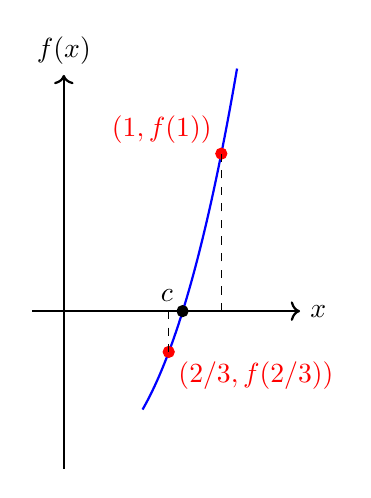
\begin{tikzpicture}[scale=2]
    % Axes
    \draw[->, thick] (-0.2, 0) -- (1.5, 0) node[right] {$x$};
    \draw[->, thick] (0, -1) -- (0, 1.5) node[above] {$f(x)$};
    
    % Curve
    \draw[domain=0.5:1.1, smooth, variable=\x, blue, thick] plot ({\x}, {\x*\x*\x + \x*\x - 1});
    
    % Points
    \filldraw[red] (0.666, -0.259) circle (1pt) node[below right] {$(2/3, f(2/3))$};
    \filldraw[red] (1, 1) circle (1pt) node[above left] {$(1, f(1))$};
    
    % Root
    \filldraw[black] (0.754, 0) circle (1pt) node[above left] {$c$};
    
    % Dashed lines
    \draw[dashed] (0.666, 0) -- (0.666, -0.259);
    \draw[dashed] (1, 0) -- (1, 1);
\end{tikzpicture}
\end{center}

\subsection{Heuristics \& "Cheats"}
\begin{itemize}
    \item \textbf{The "Zero" Trap:} When a problem asks for "nonzero real numbers," immediately check if your algebraic manipulation accidentally assumed division by zero or if the only solution is zero (as in 5.45).
    \item \textbf{Prime Sieving:} If a problem asks to prove primes of a certain form do not exist, immediately check modulo 2, 3, 5, and 7. One of these will almost always force a composite number.
\end{itemize}

\subsection{Pitfalls \& Fallacies}
\begin{itemize}
    \item \textbf{Proof by Example for Universals:} You can prove $\exists x, P(x)$ with one example. You \textit{cannot} prove $\forall x, P(x)$ with one example.
    \item \textbf{Assuming the Supremum is in the Set:} When proving existence of a maximum, do not assume $\sup(S) \in S$ unless $S$ is closed.
\end{itemize}

\newpage

% ==========================================
% PART 5: CONCEPTUAL SYNTHESIS
% ==========================================
\section{Part 5: Conceptual Synthesis and The "Big Picture"}

\subsection{A) Thematic Connections}
The core theme of this chapter is \textbf{formalizing the boundaries of mathematical truth}. By mastering existence and non-existence proofs, we transition from computation to epistemology—understanding \textit{how} we know a mathematical object can or cannot exist. This unifies previous topics in logic (De Morgan's Laws) with algebraic structures (modular arithmetic) and analysis (continuity).

\subsection{B) Forward and Backward Links}
\begin{itemize}
    \item \textbf{Backward Links:} This chapter relies heavily on the Law of Excluded Middle ($P \lor \sim P$) established in basic propositional logic. Disproving existence is the ultimate application of Proof by Contradiction.
    \item \textbf{Forward Links:} Understanding non-constructive existence is the bedrock of \textbf{Measure Theory} and \textbf{Topology}. For example, the existence of non-Lebesgue measurable sets relies entirely on the Axiom of Choice (a non-constructive existence axiom). In topology, Brouwer's Fixed Point Theorem guarantees the existence of a fixed point without telling you how to find it, which is crucial for proving the existence of Nash Equilibria in Game Theory.
\end{itemize}

% ==========================================
% PART 6: ABSTRACT REAL-WORLD MODELING
% ==========================================
\section{Part 6: Abstract Real-World Modeling (AI, ML, \& Quant Finance)}

\subsection{A) Concrete Scenarios}
\begin{enumerate}
    \item \textbf{Quantitative Finance (Arbitrage Pricing Theory):} The First Fundamental Theorem of Asset Pricing states that a market is free of arbitrage \textit{if and only if} there \textbf{exists} an Equivalent Martingale Measure (Risk-Neutral Measure). This is a pure existence theorem.
    \item \textbf{Machine Learning (Loss Landscapes):} In overparameterized neural networks, researchers must prove the \textbf{existence} of a global minimum that perfectly interpolates the training data, often relying on non-constructive topological proofs.
\end{enumerate}

\subsection{B) Model Problem Setup: The Existence of a Risk-Neutral Measure}
Let us formalize the existence of a risk-neutral measure in a one-period binomial market model.
\begin{definition}[Market Model]
    Let the state space be $\Omega = \{\omega_1, \omega_2\}$ representing an "up" or "down" market. Let $\Prob$ be the real-world probability measure where $\Prob(\omega_1) > 0$ and $\Prob(\omega_2) > 0$.
    Let $B$ be a risk-free bond with $B_0 = 1$ and $B_1 = 1+r$.
    Let $S$ be a risky stock with $S_0 = s$. At time $t=1$, $S_1(\omega_1) = u \cdot s$ and $S_1(\omega_2) = d \cdot s$, where $u > 1+r > d$.
\end{definition}

\textbf{Theorem to Prove:} \textit{There exists a unique equivalent probability measure $\Q \sim \Prob$ such that the discounted stock price is a martingale under $\Q$.}

\begin{proof}[Proof of Existence]
    We must prove $\exists \Q$ such that $\Q(\omega_1) = q > 0$, $\Q(\omega_2) = 1-q > 0$, and $\E^\Q\left[\frac{S_1}{1+r}\right] = S_0$.
    Set up the martingale condition:
    \[ \frac{1}{1+r} [q(u \cdot s) + (1-q)(d \cdot s)] = s \]
    Divide by $s$:
    \[ q \cdot u + (1-q) \cdot d = 1+r \]
    \[ q(u-d) = 1+r-d \implies q = \frac{1+r-d}{u-d} \]
    Since $u > 1+r > d$, we have $1+r-d > 0$ and $u-d > 0$. Furthermore, $u - (1+r) > 0 \implies q < 1$.
    Thus, $0 < q < 1$. 
    We have constructively proven the \textbf{existence} of the risk-neutral measure $\Q$. This guarantees the market is arbitrage-free.
\end{proof}

\newpage

% ==========================================
% PART 7: COMMON VARIATIONS
% ==========================================
\section{Part 7: Common Variations and Untested Concepts}

A common variation not heavily tested in the provided homework is proving the \textbf{existence of a limit} using the formal $\epsilon-\delta$ definition, which is an existence proof with nested quantifiers: $\forall \epsilon > 0, \exists \delta > 0, \forall x \dots$

\textbf{Example Variation:} Prove that $\lim_{x \to 2} (3x - 1) = 5$.
\begin{proof}
    We must show: $\forall \epsilon > 0, \exists \delta > 0$ such that if $0 < |x - 2| < \delta$, then $|(3x - 1) - 5| < \epsilon$.
    Let $\epsilon > 0$ be arbitrary. 
    We need $|3x - 6| < \epsilon \implies 3|x - 2| < \epsilon \implies |x - 2| < \frac{\epsilon}{3}$.
    \textbf{Constructive Existence of $\delta$:} Choose $\delta = \frac{\epsilon}{3}$. Since $\epsilon > 0$, $\delta > 0$.
    Assume $0 < |x - 2| < \delta$. Then:
    \[ |(3x - 1) - 5| = |3x - 6| = 3|x - 2| < 3\delta = 3\left(\frac{\epsilon}{3}\right) = \epsilon \]
    Thus, the limit exists and equals 5.
\end{proof}

% ==========================================
% PART 8: ADVANCED DIAGNOSTIC TESTING
% ==========================================
\section{Part 8: Advanced Diagnostic Testing: "Find the Flaw"}

Below are five proofs containing a single, subtle logical flaw. Can you find them?

\textbf{Problem 1:} Prove that there exists a maximum element in the open interval $(0, 1)$.
\begin{proof}[Flawed Proof]
    Let $S = (0, 1)$. The set $S$ is non-empty and bounded above by 1. By the Axiom of Completeness for the real numbers, every non-empty subset of $\R$ that is bounded above has a supremum. Let $M = \sup(S)$. Since $M$ is the least upper bound, it is the maximum value of the set. Thus, a maximum exists.
\end{proof}

\textbf{Problem 2:} Prove that there exists a unique real root to the equation $x^2 + 1 = 0$.
\begin{proof}[Flawed Proof]
    Let $f(x) = x^2 + 1$. To find the roots, we take the derivative $f'(x) = 2x$. Setting the derivative to zero gives $2x = 0 \implies x = 0$. Since there is exactly one critical point, the function can cross the x-axis at most once. Thus, if a root exists, it is unique.
\end{proof}

\textbf{Problem 3:} Disprove the statement: $\exists x \in \R$ such that $x^3 - x = 0$.
\begin{proof}[Flawed Proof]
    Assume such an $x$ exists. Then $x^3 - x = 0 \implies x(x^2 - 1) = 0$. Dividing both sides by $x$ yields $x^2 - 1 = 0$, which means $x = 1$ or $x = -1$. However, if we plug $x=0$ into the original equation, we get $0 = 0$. This contradicts our derived solutions of $1$ and $-1$. Thus, no such $x$ exists.
\end{proof}

\textbf{Problem 4:} Prove that there exist irrational numbers $a$ and $b$ such that $a+b$ is rational.
\begin{proof}[Flawed Proof]
    Let $a = \sqrt{2}$ and $b = \sqrt{3}$. Both are irrational. Assume for contradiction that $a+b = r$, where $r$ is rational. Then $\sqrt{2} + \sqrt{3} = r$. Squaring both sides gives $5 + 2\sqrt{6} = r^2$. Rearranging yields $\sqrt{6} = \frac{r^2 - 5}{2}$. Since $r$ is rational, the right side is rational, implying $\sqrt{6}$ is rational, which is a contradiction. Thus, $a+b$ is rational.
\end{proof}

\textbf{Problem 5:} Prove that there exists a real number $x$ such that $e^x < 0$.
\begin{proof}[Flawed Proof]
    By Euler's Identity, we know that $e^{i\pi} + 1 = 0$. Rearranging this gives $e^{i\pi} = -1$. Let $x = i\pi$. Then $e^x = -1$, and since $-1 < 0$, we have found an $x$ such that $e^x < 0$.
\end{proof}

\hrulefill

\subsection*{Solution Key to Diagnostic Tests}
\begin{enumerate}
    \item \textbf{Flaw:} The supremum of a set is not necessarily an element of the set. $\sup(0, 1) = 1$, but $1 \notin (0, 1)$, so it is not a maximum.
    \item \textbf{Flaw:} The proof successfully proves uniqueness \textit{if} a root exists, but it completely skips the existence proof. In fact, $x^2+1=0$ has no real roots.
    \item \textbf{Flaw:} Dividing by $x$ implicitly assumes $x \neq 0$. You cannot divide by a variable without checking the zero case. The statement is actually true ($x=0, 1, -1$ are all valid).
    \item \textbf{Flaw:} The proof successfully shows that $\sqrt{2}+\sqrt{3}$ is \textit{irrational}, which is the exact opposite of what was requested. To prove the prompt, one should choose $a = \sqrt{2}$ and $b = -\sqrt{2}$, yielding $a+b = 0 \in \Q$.
    \item \textbf{Flaw:} The prompt asks for a \textit{real} number $x \in \R$. The value $x = i\pi$ is a complex number, so it is outside the specified domain.
\end{enumerate}

\end{document}